\documentclass[twoside]{article}
\usepackage{graphicx}
\usepackage[a4paper]{geometry}
\usepackage[utf8]{inputenc} 
\usepackage{xcolor}
\usepackage{hyperref}
\hypersetup{
    colorlinks = true,
    linkcolor = teal,
    citecolor = blue
}

% use mathematical packages
\usepackage{amsmath, amssymb}
\usepackage{makecell}


\pagestyle{empty}

\geometry{tmargin=3cm, bmargin=3cm, lmargin=3cm, rmargin=3cm}
\setlength\parindent{0pt}
\begin{document}

\begin{flushright}

\includegraphics[angle=0,keepaspectratio,width=3cm]{logo.pdf}
\end{flushright}

\noindent {\small \textsl{IX Xornada de Usuarios de R en Galicia\textsl{\ \newline Santiago de Compostela}, 20 de outubro do 2022}} \vspace{20pt}

\begin{center}
\textbf{Automatic covariates selection in dynamic regression models with application to COVID-19 evolution}

\vspace{0.15cm}

Ana Ezquerro$^{1}$, Germán Aneiros$^{2}$, Manuel Oviedo$^{3}$
\end{center}

\vspace{0.06cm}

$^{1}$University of A Coruña, \texttt{ana.ezquerro@udc.es}

$^{2}$CITIC, Grupo MODES, Departamento de Matemáticas, University of A Coruña, \texttt{german.aneiros@udc.es}


$^{3}$CITIC, Grupo MODES, Departamento de Matemáticas, University of A Coruña, \texttt{manuel.oviedo@udc.es}


\begin{center}
\textbf{Abstract}
\end{center}


\begin{quotation}
    This work introduces a new approach in time-series analysis field for automatic covariates selection in dynamic regression models. Based on \cite{cryer2008time} and \cite{hyndman2018forecasting} previous study, a forward-selection method is proposed for adding new significant covariates from a given set. This algorithm has been implemented and optimized in R as a package, and we openly publish its sources in order to make it available for all the R community. Our method has been applied to multiple simulations to validate its performance. Finally, the obtained results from the IRAS database of Catalonia are presented to analyze the COVID-19 evolution. 
\end{quotation}

\vspace{0.4cm}

\textbf{Keywords}: Time series, dynamic regression models, selection methods, forecasting.

\vspace{0.4cm}

\begin{center}
\textbf{Introduction}
\end{center}


In time-series analysis, the well-known dynamic regression models allow formally modelling the dependence between a set of covariates and a dependent variable considering the intrinsic temporal component of all participant variables. Thus, this type of regression models are of widespread application in diverse scenarios where it is desired to analyze the effect of recollected data in a time series of interest. 

Formally, dynamic linear regression models define the linear dependence between a stochastic process $Y_t$ (the dependent variable) and a set of processes  $\mathcal{X}=\{ X_t^{(1)}, X_t^{(2)}, ..., X_t^{(m)}\}$ (candidates for regressor variables) in times non-greater than $t$:

\begin{equation}\label{dynamic.regression.model}
Y_t = \beta_0 + \beta_1 X^{(1)}_{t-r_1} + \beta_2 X^{(2)}_{t-r_2} + \cdots + \beta_m  X^{(m)}_{t-r_m} + \eta_t 
\end{equation}

\noindent where $r_i \geq 0$, for $i=1,...,m$, and $\eta_t \sim$ ARMA(p,q).

In this work we formally introduce a new algorithm to select covariates which significantly influence the behavior of a dependent variable. The implementation of this selection method is publicly available.




\begin{center}
\textbf{Methodology}
\end{center}

Following the definition in \ref{dynamic.regression.model}, \cite{cryer2008time} proposed a method named \textit{prewhitening} for removing spurious correlation (false linear correlation) between two processes $X_t$ and $Y_t$ (where one of them is not white noise and/or the other is not stationary) by analyzing the cross correlation function $\rho_k(\ddot{X}_t, \ddot{Y}_t) =  \cfrac{\text{Cov}(\ddot{X}_t, \ddot{Y}_{t-k})}{\sigma_{\ddot{X}_t} \sigma_{\ddot{Y}_t}} $ where $\sigma_{Z_t}$ denotes the standard deviation of a stochastic process $Z_t$ and $\ddot{X}_t$ and $\ddot{Y}_t$ are obtained via some linear filter application to $X_t$ and $Y_t$ ensuring one of them is white noise and the other is a stationary process. Specifically, \cite{cryer2008time} proposes a real linear correlation between $X_t$ and $Y_t$ if exists some $k$ where $\rho_k(\ddot{X}_t, \ddot{Y}_t)$ is statistically significant. This method is applied to obtain the optimal lags of each regressor in \ref{dynamic.regression.model}, considering the condition of $k$ being less or equal than $0$.

Our approach iteratively adds dependent processes to a model by checking if a significant correlation (as in \cite{cryer2008time}) exists between a new process (candidate for regressor variable) and the residuals $\eta_t$ of a simpler model.

Let $Y_t$ be the stochastic dependent process and $\mathcal{X}$ be the set of processes that might act as regressor variables in the model (candidates), and an information criterion (IC) for model evaluation. Our method proceeds as follows:


\begin{enumerate}
    \item Initialization. Consider the process $\tilde{Y}_t=Y_t$ that will be used to check the existence of linear correlation between $Y_t$ and each $X_t\in \mathcal{X}$ with \cite{cryer2008time} method, $\nu=\infty$ the value of the IC corresponding to the best model with \ref{dynamic.regression.model} form, $\mathcal{X}^{(s,r)}$ the set of selected covariates paired with their respective optimal lags and $\mathcal{X}^{(s)}$ the set of selected covariates (with no lag information). Let $\mathcal{M}(\mathcal{Z})$ be the fitted dynamic regression model regarding $Y_t$ where $\mathcal{Z}$ is the set of covariates paired with their optimal lags:
    \[ \mathcal{M}(\mathcal{Z}) := Y_t = \beta_0 + \sum_{(Z_t, r)\in\mathcal{Z}} \beta^{(Z_t, r)} Z_{t-r} + \eta_t\]
    \noindent where $\beta^{(Z_t, r)}$ is obtained via some estimation.

    \item Iterative selection. For each $X_t\in\mathcal{X}-\mathcal{X}^{(s)}$, obtain the optimal lag where the maximum linear cross correlation between $X_t$ and $\tilde{Y}_t$ occurs (via \cite{cryer2008time} method). Consider the process $X_t^\text{best}\in\mathcal{X}-\mathcal{X}^{(s)}$ that minimizes and improves $\nu$ value, based on the selected IC, by including it in the model with its optimal lag ($r_{X_t^\text{best}}$):
    
    \begin{equation}\label{iterative.selection}
        X^\text{best}_t =  \underset{X_t\in\mathcal{X}-\mathcal{X}^{(s)}}{\arg\min} \Bigg\{ \ \text{criteria}\Bigg(\ \mathcal{M}\Big(\mathcal{X}^{(s,r)} \cup \big\{(X_t, r_{X_t})\big\} \Big) \ \Bigg) \Bigg\}
    \end{equation}

    \noindent conditioned to $\text{criteria}(\cdot) < \nu$\footnote{for simplicity, we denote the expression in $\text{criteria}()$ in \ref{iterative.selection} as $\cdot$}. 
    If $X^{\text{best}}_t$ exists, consider $\mathcal{X}^{(s,r)} = \mathcal{X}^{(s,r)}  \cup \{(X_t^\text{best}, r_{X_t^\text{best}})\}$, $\tilde{Y}_t = \eta_t$ and $\nu=\text{criteria}(\mathcal{X}^{(s,r)})$\footnote{once $X_t^\text{best}$ has been added to the model }. Repeat this step until no process $X_t\in\mathcal{X}-\mathcal{X}^{(s)}$ can be added to the model, i.e. $X_t^\text{best}$ does not exist.

    \item Finalization. If the errors $\eta_t$ of $\mathcal{M}(\mathcal{X}^{(s,r)})$ are not stationary and no model with $\eta_t\sim\text{ARMA(p,q)}$ and $\mathcal{X}^{(s,r)}$ covariates can be adjusted, consider the regular differentiation of all data (dependent variable and regressor candidates) and return to (1). Otherwise, it is proven that  $\mathcal{M}(\mathcal{X}^{(s,r)})$ with stationary errors defines the significant correlation between the set of $\mathcal{X}^{(s)}$ regressor variables and the dependent process $Y_t$.
\end{enumerate}

This algorithm was implemented in R programming language. The step 2 was optimized by parallelizing the fit of independent models of each candidate in $\mathcal{X}$.  Dickey-Fuller test is used for checking processes stationary, Ljung-Box to check the independence, Shapiro-Wilks and Jarque-Bera tests for normality and t-test for zero mean of ARIMA residuals. 

\begin{center}
    \textbf{Simulation results}
\end{center}

In order to validate the performance of our selection method, we simulate multiple scenarios where a time series $Y_t$ was artificially constructed with other variables (introduced with their respective coefficients and lags as in \ref{dynamic.regression.model}), which were added to a set of candidates along with more variables which do not influence in the construction of $Y_t$. The algorithm was tested when the residuals of the model $\eta_t$ were stationary and non-stationary. 

Specifically, we simulate $M=200$ times the following scenario: 
\begin{enumerate}
    \item We generate seven different independent time series (each modelable by an ARIMA), of which six of them act as the covariate candidates set: $\mathcal{X} = \{ X_t^{(1)}, X_t^{(2)}, ..., X_t^{(6)} \}$; and the remaining as the residuals $\eta_t$ of the model.
    \item We construct the dependent variable $Y_t$ by a linear combination of $\{ X_t^{(1)}, X_t^{(2)}, X_t^{(3)} \}$, randomly lagged $r=0,...,6$ moments  (where the coefficients are randomly generated), with an intercept $\beta_0$ and the generated residuals $\eta_t$. Formally,
    \[ Y_t = \beta_0  + \beta_1 X_{t-r_1}^{(1)} + \beta_2 X_{t-r_2}^{(2)} + \beta_3 X_{t-r_3}^{(3)} + \eta_t \]
    where $\beta_0,... \beta_3$ are randomly generated, and $r_i \in [0, 6]$ for $i=1,2,3$.
    \item We launch our selection method with different configurations:
    \begin{itemize}
        \item Using as the information criterion the AIC, BIC and AICc.
        \item Using as the method to check stationary the Dickey-Fuller test or via analyzing the differentiation order when an ARIMA is adjusted.
    \end{itemize}
    \item Evaluate the selection method using as metrics the percentage of times a covariate is:
    \begin{enumerate}
        \item correctly added to the model (\textit{true positive}),
        \item incorrectly added to the model (\textit{false positive}),
        \item correctly not added to the model (\textit{true negative}),
        \item incorrectly not added to the model (\textit{false negative}).
    \end{enumerate}
\end{enumerate}





\begin{figure}
    \caption{Example of code output and results of \texttt{auto.fit.arima.regression()} when running the selection method}
    \label{simulation.example}
    \vspace{0.3em}
    \fbox{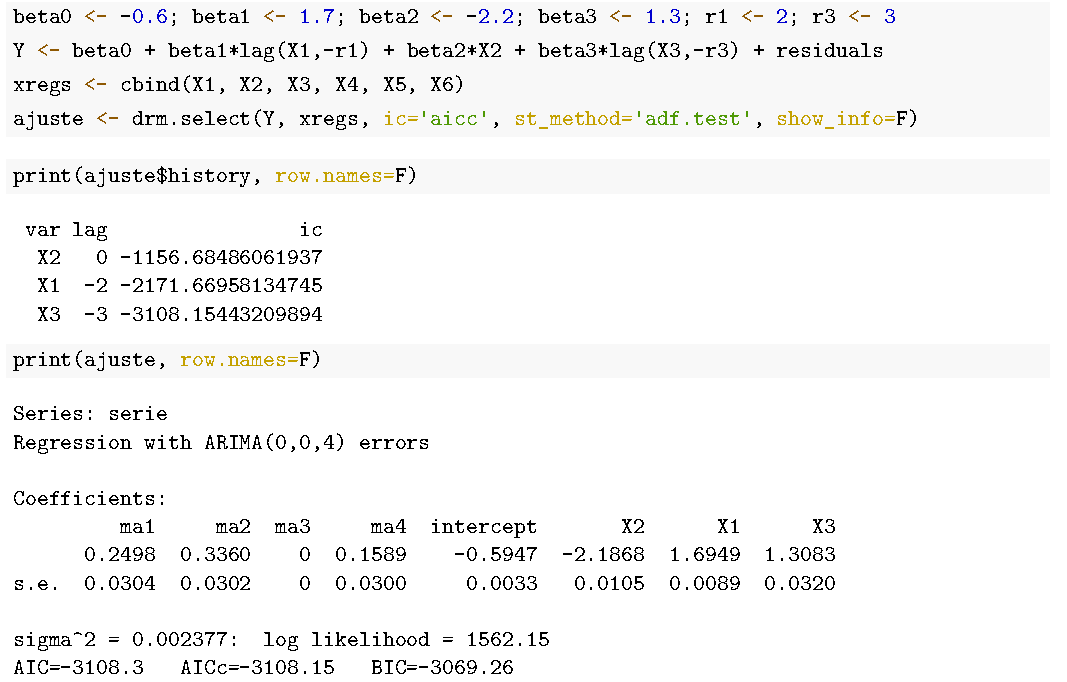
\includegraphics[scale=0.8]{simulation-example.pdf}}
\end{figure}


Figure \ref{simulation.example} displays the result of calling the function that implements the selection method. The DataFrame stored in \texttt{\$history} provide information about the covariates iteratively added to the model, the IC value achieved and the lag they were added with. When printing the resultant object (\texttt{ajuste}) we see that the estimated regression coefficients are nearly the same than the real values artificially set. Also, the lags estimated by the method are correct, and the errors of the final model are stationary.

Table illustrates a resume of the results of our approach when running our approach $M=200$ times with different configurations and using stationary an non-stationary errors.






\begin{center}
\textbf{Application to COVID19 evolution}
\end{center}



Due to the impact of COVID-19 around the world, we use this method to formalize and study the relation of the COVID-19 evolution in Catalonia (Spain) with the flu syndrome, COVID-19 vaccination and other recollected variables from the IRAS database. Individual data was aggregated by age ranges and Health Areas to study the correlation between groups and their influence in the global evolution. 



\begin{table}
    \centering\small
    \setlength{\tabcolsep}{10pt}
    \caption{Information about the dynamic regression model constructed via selection of multiple vaccination variables to model COVID19 evolution} 
    \label{covid19model}

    \vspace{0.5em}
    \begin{tabular}{|l|cc|}
        \hline
        \textbf{Covariate}  & \textbf{Lag}  & \textbf{Coefficient est. (s.e)} \\ 
        \hline 
        \texttt{vac4565}    & -3            & -0.0410 (0.0057)                      \\ 
        \texttt{vac6580}    & -2            & -0.0468 (0.0120)                      \\
        \texttt{vac1845}    & -6            & -0.0901 (0.0047)                      \\
        \hline
        \texttt{vac1218}    & \multicolumn{2}{c|}{Not included in the model} \\
        \texttt{vac80}      & \multicolumn{2}{c|}{Not included in the model} \\
        \hline
        residuals           & ARIMA(4, 0, 0) & \makecell[c]{$\phi_1=2.0816 (0.0810)$ \\ $\phi_2=-1.2837 (0.1152)$ \\ $\phi_4=0.1919 (0.0432)$ } \\
        \hline
    \end{tabular}
\end{table}    

Table \ref{covid19model} resumes the algorithm trace and the order of covariates addition to the model. The covariates named \texttt{vac1218}, \texttt{vac1845}, \texttt{vac4565}, \texttt{vac6580} correspond the vaccination data in population from 12, 18, 45 and 65 up to 18, 45, 65 and 80 years old (exclusive), and \texttt{vac80} corresponds the vaccination in population from 80 years. We can analyze the vaccination has a negative impact in the expansion of COVID19, specifically, the vaccination of working-age population. 

\begin{center}
    \textbf{Future work}
\end{center}
Our approach has considered DRM covariates modelable by ARIMA models, which successfully covers a wide real-life applications. However, other cases might be considered, such as adding functional variables and discrete variables to the set of candidates. 

\begin{center}
    \textbf{Acknowledgements}
\end{center}
To Banco Santander for the scholarships offered in 2021/2022, which helped the investigation of this proposal, and to \textit{Departamento de Matemáticas} of University of A Coruña.


\bibliographystyle{plain}
\bibliography{bibliography}




\end{document}
